%% Exemplo de utilizacao do estilo de formatacao abnt-UTFPR.cls para LaTeX (v1.3)
%% Autores: Hugo Vieira Neto (hvieir@utfpr.edu.br)
%%          Diogo Rosa Kuiaski (diogo.kuiaski@gmail.com)

\documentclass{abnt-UTFPR} % estilo de documento abnTeX
\usepackage[alf,abnt-emphasize=bf,bibjustif,recuo=0cm]{abntcite} % estilo de bibliografia abnTeX
\usepackage[brazil]{babel} % pacote portugues brasileiro
%\usepackage[latin1]{inputenc} % pacote para acentuacao direta
\usepackage{amsmath,amsfonts,amssymb} % pacote matematico
\usepackage{graphicx} % pacote grafico
\usepackage{times} % fonte times


% ---------- Preambulo ----------
\instituicao{Universidade Tecnol\'ogica Federal do Paran\'a} % nome da instituicao
\departamento{Departamento Acad\^emico de Eletr\^onica} % nome do departamento
\programa{Curso Superior de Tecnologia em Mecatr\^onica Industrial} % nome do curso

\documento{Trabalho de Conclus\~ao de Curso} % [Trabalho de Conclus\~ao de Curso] ou [Relat\'orio de Est\'agio]
\titulacao{Tecn\'ologo} % [T\'ecnico], [Tecn\'ologo] ou [Engenheiro]

\titulo{T\'itulo em Portugu\^es} % titulo do trabalho em portugues
\title{Title in English} % titulo do trabalho em ingles

\autor{Nome do Primeiro Autor} % primeiro autor do trabalho
\autordois{Nome do Segundo Autor} % segundo autor do trabalho, caso exista
%\autortres{Nome do Terceiro Autor} % terceiro autor do trabalho, caso exista
%\autorquatro{Nome do Quarto Autor} % quarto autor do trabalho, caso exista
\cita{SOBRENOME 1, Nome 1; SOBRENOME 2, Nome 2} % sobrenome (maiusculas) e nome do(s) autor(es) do trabalho, separados por ponto-e-virgula (ate quatro autores para TCC)

\palavraschave{Palavra-chave 1, Palavra-chave 2, ...} % palavras-chave do trabalho
\keywords{Keyword 1, Keyword 2, ...} % palavras-chave do trabalho em ingles

\comentario{\UTFPRdocumentodata\ apresentado ao \UTFPRdepartamentodata\ como requisito parcial para obten\c{c}\~ao do grau de \UTFPRtitulacaodata\ no \UTFPRprogramadata\ da \ABNTinstituicaodata.}

\orientador{Nome do Orientador} % nome do orientador do trabalho
%\orientador[Orientadora:]{Nome da Orientadora} % <- no caso de orientadora, usar esta sintaxe
\coorientador{Nome do Co-orientador} % nome do co-orientador do trabalho, caso exista
%\coorientador[Co-orientadora:]{Nome da Co-orientadora} % <- no caso de co-orientadora, usar esta sintaxe

\local{Curitiba} % cidade
\data{2009} % ano


%---------- Inicio do Documento ----------
\begin{document}

\capa % geracao automatica da capa
\folhaderosto % geracao automatica da folha de rosto
%\termodeaprovacao % <- ainda a ser implementado corretamente

% dedicat�ria (opcional)
\begin{dedicatoria}
Texto da dedicat\'oria.
\end{dedicatoria}

% agradecimentos (opcional)
\begin{agradecimentos}
Texto dos agradecimentos.
\end{agradecimentos}

% epigrafe (opcional)
\begin{epigrafe}
Texto da ep\'igrafe.
\end{epigrafe}

%resumo
\begin{resumo}
Texto do resumo (m\'aximo de 500 palavras).
\end{resumo}

%abstract
\begin{abstract}
Abstract text (maximum of 500 words).
\end{abstract}

% listas (opcionais, mas recomenda-se a partir de 5 elementos)
\listadefiguras % geracao automatica da lista de figuras
\listadetabelas % geracao automatica da lista de tabelas
\listadesiglas % geracao automatica da lista de siglas
\listadesimbolos % geracao automatica da lista de simbolos

% sumario
\sumario % geracao automatica do sumario


%---------- Inicio do Texto ----------
% recomenda-se a escrita de cada capitulo em um arquivo texto separado (exemplo: intro.tex, fund.tex, exper.tex, concl.tex, etc.) e a posterior inclusao dos mesmos no mestre do documento utilizando o comando \input{}, da seguinte forma:
%\input{intro.tex}
%\input{fund.tex}
%\input{exper.tex}
%\chapter{Conclus�o}

O presente trabalho de conclus�o de curso apresentou objetivos abrangentes, envolvendo desenvolvimento de hardware e software. No contexto da navega��o rob�tica, surgiu a necessidade de se utilizar um rob� real com a finalidade de se obter resultados mais significativos. Desse modo, foi elaborado um projeto cujo escopo tamb�m foi reconstruir e adequar uma plataforma rob�tica previamente dispon�vel, que � descrita na sec��o \ref{sec:estpro}, por�m que n�o estava em condi��es de uso imediato. A equipe procedeu com testes em laborat�rio de eletr�nica afim de avaliar as condi��es iniciais do rob�, conforme � descrito na sec��o \ref{sec:testecomp}. Uma an�lise de software foi efetuada e o c�digo original do microcontrolador C8051F340DK, disponibilizado como parte integrante do rob� Bellator \cite{BELLATOR}, foi avaliado e reconfigurado de acordo com as necessidades do projeto, o que � descrito em detalhes na se��o \ref{sec:codmicro}. Havendo necessidade de implementa��o de hardware, a equipe projetou e construiu uma placa de roteamento para alimentar os sensores e encoders, assim como tratar os sinais destes e os de PWM, como � descrito na se��o \ref{sec:desroteamento}. Finalmente, o hardware acoplado foi configurado e o software que executou os algortimos de navega��o foi desenvolvido, conforme a se��o \ref{sec:ts}. Com isso, a equipe concluiu a primeira parte do projeto, a qual consistiu na reconstru��o e adequa��o do rob� Bellator.

Estando a plataforma rob�tica funcional, seguiram-se o projeto e implementa��o dos algoritmos de navega��o propostos. A L�gica Fuzzy foi estudada e apresentada na se��o \ref{sec:logfuzzy} e a metodologia de Mapas Cognitivos Fuzzy (FCM) foi estudada e apresentada na se��o \ref{sec:fcm}. Com a teoria fundamentada, a equipe projetou os algoritmos e implementou-os na linguagem C++, compilados para executar no hardware acoplado, placa TS-7260. O projeto e a implementa��o dos algoritmos de navega��o Fuzzy e FCM s�o descritos em detalhes nas se��es \ref{sec:algfuzzy} e \ref{sec:algedfcm}, respectivamente. Ap�s a implementa��o, a equipe submeteu os algoritmos a uma s�rie de testes b�sicos, denominada Testes Iniciais, que serviram para fornecer a primeira realimenta��o do projeto dos algoritmos e pode ser lido na se��o \ref{sec:testesini}. Finalizados esses testes, foram elaborados testes complexos, denominados Testes Avan�ados, para estressar os sistemas de navega��o propostos e fornecer a segunda realimenta��o do projeto dos algoritmos, conforme � descri��o na se��o \ref{sec:testesavan}. Finalmente, ap�s os testes avan�ados, os algoritmos resolviam problemas complexos de navega��o, como o corredor sem sa�da e o problema de decis�o quando dois obst�culos laterais e um frontal era colocado diante do rob�, e poderiam ser usados nos testes finais, que forneceram os dados para a an�lise de resultados e foram denominados Testes Comparativos, conforme � descrito na se��o \ref{sec:testescomp}. Com isso foi conclu�do outros dois objetivos do projeto, que foram o projeto e implementa��o dos algoritmos de navega��o e a elabora��o e execu��o de uma metodologia de testes comparativos entre os algoritmos.

Para trabalhos futuros utilizando a plataforma Bellator reconstru�da, a equipe recomenda combinar sensores de ultra-som ao sensores infra vermelho, justificando isso porque os sensores de ultra-som apresentam uma faixa de opera��o cuja dist�ncia m�nima � menor que a do infra-vermelho, podendo capturar dist�ncias de 2 cm. Atualmente a dist�ncia m�nima suportada pelo sistema de navega��o � de 15 cm, com os sensores de ultra-som, os algoritmos poderiam operar em uma faixa mais abrangente. Outra sugest�o � introduzir ao sistema uma realimenta��o por b�ssola pois nesse projeto a realimenta��o odom�trica fornecida pelos encoders � utilizada para ajustar a velocidade das rodas e n�o faz uma interpreta��o da dire��o do rob�. Para tornar o rob� seguro para o manuseio, sugere-se a fixa��o dos sensores parafusando-os no chassi do Bellator e acoplando uma casca que proteja os circuitos microcontrolados. A equipe tamb�m recomenda a reconstru��o da placa de roteamento utilizando um m�todo industrial para confecc��o de placas de circuito impresso. Para os sistemas de navega��o, um trabalho futuro de grande riqueza seria introduzir ao sistema a capacidade de interpretar a posi��o do rob� em rela��o a um referencial. Com isso, o rob� seria capaz de resolver problemas nos quais este deve partir de um ponto inicial no espa�o a um ponto final, guiando-se pelos sensores para evitar colis�es e realimentar-se por um sistema de posicionamento para corrigir a traget�ria. Outro trabalho, produto deste, seria introduzir ao sistema uma mem�ria a qual pudesse mapear os obst�culos capturados pelos sensores do rob�, assim sendo, produzir-se-ia um artefato aut�nomo capaz de mapear terrenos. Outro aprimoramento da plataforma seria implementar um sistema de controle remoto por joystick, na qual uma base remota podesse pilotar o rob� via joystick. Finalmente, a equipe sugere um projeto futuro no qual seja implementado um sistema de vis�o computacional por c�mera de v�deo.

A equipe concluiu esta monografia justificando que os objetivos descritos na introdu��o, se��o \ref{rec:obj}, foram alcan�ados e est�o de acordo com os requisitos m�nimos de um curso de Engenharia de Computa��o. Os problemas encontrados na execu��o do projeto est�o associados ao escopo abrangente do mesmo, o qual envolveu o desenvolvimento de hardware e software em um projeto integrador. A subdivis�o do projeto em diversos objetivos, sendo um pr�-requisito para o outro, foi inevit�vel para alcan�ar os resultados finais. A equipe encontrou dificuldades durante a reconstru��o do rob�, configura��o da placa TS-7260, testes integrados de funcionamento do rob�, implementa��o dos algoritmos, execu��o dos testes dos algoritmos e an�lise de resultados. Durante a recontru��o, os componentes eletr�nicos foram testados isoladamente e houve riscos de haver danos, o que representaria atrasos no projeto. A placa TS-7260 apresentou complexidade para ser configurada pois n�o houve um t�cnico dispon�vel para auxiliar a equipe, a qual teve que aprender a trabalhar com esse hardware. Nos testes de integra��o da C8051F340DK e da TS-7260, que determinaram o funcionamento da plataforma rob�tica, foi exigido processos de depura��o integrados, nos quais os problemas foram isolados e corrigidos repetidas vezes. A implementa��o dos algoritmos at� a vers�o final, que foi utilizada nos testes comparativos, foi realizada paralelamente aos testes b�sicos e avan�ados, nas quais os problemas de navega��o foram detectados, isolados e corrigidos repetidas vezes. A metodologia de testes escolhida foi elaborada pela equipe e foram efetuados v�rios experimentos com registro em v�deo at� que se atingessem os resultados finais. Tendo com base os v�deos gravados e a experi�ncia em campo observada, a equipe precisou analisar os resultados, discut�-los e extrair conclus�es para finalizar o projeto, sendo que essa tarefa representou um trabalho cient�fico. 



%---------- Primeiro Capitulo ----------
\chapter{Introdu\c{c}\~ao}

O presente documento \'e um exemplo de uso do estilo de formata\c{c}\~ao \LaTeX\ elaborado para atender \`as Normas para Elabora\c{c}\~ao de Trabalhos Acad\^emicos da UTFPR. O estilo de formata\c{c}\~ao {\ttfamily abnt-UTFPR.cls} tem por base o pacote \textsc{abn}\TeX~-- cuja leitura da documenta\c{c}\~ao \cite{abnTeX2009} \'e fortemente sugerida~-- e o estilo de formata\c{c}\~ao \LaTeX\ da UFPR.

Para melhor entendimento do uso do estilo de formata\c{c}\~ao {\ttfamily abnt-UTFPR.cls}, aconselha-se que o potencial usu\'ario analise os comandos existentes no arquivo \TeX\ ({\ttfamily modelo\_*.tex}) e os resultados obtidos no arquivo PDF ({\ttfamily modelo\_*.pdf}) depois do processamento pelo software \LaTeX\ + \textsc{Bib}\TeX~\cite{LaTeX2009,BibTeX2009}. Recomenda-se a consulta ao material de refer\^encia do software para a sua correta utiliza\c{c}\~ao~\cite{Lamport1986,Buerger1989,Kopka2003,Mittelbach2004}.

\section{Motiva\c{c}\~ao}

Uma das principais vantagens do uso do estilo de formata\c{c}\~ao {\ttfamily abnt-UTFPR.cls} para \LaTeX\ \'e a formata\c{c}\~ao \textit{autom\'atica} dos elementos que comp\~oem um documento acad\^emico, tais como capa, folha de rosto, dedicat\'oria, agradecimentos, ep\'igrafe, resumo, abstract, listas de figuras, tabelas, siglas e s\'imbolos, sum\'ario, cap\'itulos, refer\^encias, etc. Outras grandes vantagens do uso do \LaTeX\ para formata\c{c}\~ao de documentos acad\^emicos dizem respeito \`a facilidade de gerenciamento de refer\^encias cruzadas e bibliogr\'aficas, al\'em da formata\c{c}\~ao~-- inclusive de equa\c{c}\~oes  matem\'aticas~-- correta e esteticamente perfeita.

\section{Objetivos}

\subsection{Objetivo Geral}

Prover um modelo de formata\c{c}\~ao \LaTeX\ que atenda \`as Normas para Elabora\c{c}\~ao de Trabalhos Acad\^emicos da UTFPR~\cite{UTFPR2008} e \`as Normas de Apresenta\c{c}\~ao de Trabalhos Acad\^emicos do DAELN~\cite{DAELN2006}.

\subsection{Objetivos Espec\'ificos}

\begin{itemize}
	\item Obter documentos acad\^emicos automaticamente formatados com corre\c{c}\~ao e perfei\c{c}\~ao est\'etica.
	\item Desonerar autores da tediosa tarefa de formatar documentos acad\^emicos, permitindo sua concentra\c{c}\~ao no conte\'udo do mesmo.
	\item Desonerar orientadores e examinadores da tediosa tarefa de conferir a formata\c{c}\~ao de documentos acad\^emicos, permitindo sua concentra\c{c}\~ao no conte\'udo do mesmo.
\end{itemize}


%---------- Segundo Capitulo ----------
\chapter{Desenvolvimento}
\label{chap:desenv}

A seguir ilustra-se a forma de incluir figuras, tabelas, equa\c{c}\~oes, siglas e s\'imbolos no documento, obtendo indexa\c{c}\~ao autom\'atica em suas respectivas listas. A numera\c{c}\~ao sequencial de figuras, tabelas e equa\c{c}\~oes ocorre de modo autom\'atico. Refer\^encias cruzadas s\~ao obtidas atrav\'es dos comandos {\ttfamily \textbackslash label\{\}} e {\ttfamily \textbackslash ref\{\}}. Por exemplo, n\~ao \'e necess\'ario saber que o n\'umero deste cap\'itulo \'e~\ref{chap:desenv} para colocar o seu n\'umero no texto. Isto facilita muito a inser\c{c}\~ao, remo\c{c}\~ao ou reloca\c{c}\~ao de elementos numerados no texto (fato corriqueiro na escrita e corre\c{c}\~ao de um documento acad\^emico) sem a necessidade de renumer\'a-los todos.

\section{Figuras}

Na figura~\ref{fig:dummy} \'e apresentado um exemplo de gr\'afico flutuante. Esta figura aparece automaticamente na lista de figuras. Para uso avan\c{c}ado de gr\'aficos no \LaTeX, recomenda-se a consulta de literatura especializada~\cite{Goossens2007}.

\begin{figure}[!htb]
	\centering
	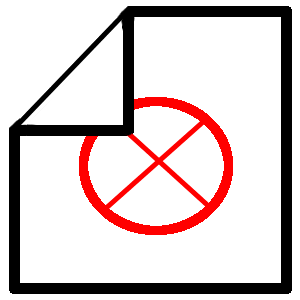
\includegraphics[width=0.2\textwidth]{./figs/dummy.png} % <- formatos PNG, JPG e PDF
	\caption[Exemplo de uma figura]{Exemplo de uma figura onde aparece uma imagem sem nenhum significado especial.}
	\fonte{\cite{abnTeX2009}}
	\label{fig:dummy}
\end{figure}

\section{Tabelas}

Tamb\'em \'e apresentado o exemplo da tabela~\ref{tab:correlacao}, que aparece automaticamente na lista de tabelas. Informa\c{c}\~oes sobre a constru\c{c}\~ao de tabelas no \LaTeX\ podem ser encontradas na literatura especializada~\cite{Lamport1986,Buerger1989,Kopka2003,Mittelbach2004}.

\begin{table}[!htb]
	\centering
	\caption[Exemplo de uma tabela]{Exemplo de uma tabela mostrando a correla\c{c}\~ao entre x e y.}
	\label{tab:correlacao}
	\begin{tabular}{cc}
		\hline 
		x & y \\
		\hline
		1 & 2 \\
		3 & 4 \\
		5 & 6 \\
		7 & 8 \\
		\hline 
	\end{tabular}
	\fonte{Autoria pr\'opria.}
\end{table}

\section{Equa\c{c}\~oes}

A transformada de Laplace \'e dada na equa\c{c}\~ao~(\ref{eq:laplace}), enquanto a equa\c{c}\~ao~(\ref{eq:dft}) apresenta a formula\c{c}\~ao da transformada discreta de Fourier bidimensional\footnote{Deve-se reparar na formata\c{c}\~ao esteticamente perfeita destas equa\c{c}\~oes!}.

\begin{equation}
X(s) = \int\limits_{t = -\infty}^{\infty} x(t) \, \text{e}^{-st} \, dt
\label{eq:laplace}
\end{equation}

\begin{equation}
F(u, v) = \sum_{m = 0}^{M - 1} \sum_{n = 0}^{N - 1} f(m, n) \exp \left[ -j 2 \pi \left( \frac{u m}{M} + \frac{v n}{N} \right) \right]
\label{eq:dft}
\end{equation}

\section{Siglas e s\'imbolos}

O pacote \textsc{abn}\TeX\ permite ainda a defini\c{c}\~ao de siglas e s\'imbolos com indexa\c{c}\~ao autom\'atica atrav\'es dos comandos {\ttfamily \textbackslash sigla\{\}\{\}} e {\ttfamily \textbackslash simbolo\{\}\{\}}. Por exemplo, o significado das siglas\sigla{CPGEI}{Programa de P\'os-gradua\c{c}\~ao em Engenharia El\'etrica e Inform\'atica Industrial},\sigla{DAELN}{Departamento Acad\^emico de Eletr\^onica} e\sigla{UTFPR}{Universidade Tecnol\'ogica Federal do Paran\'a} aparecem automaticamente na lista de siglas, bem como o significado dos s\'imbolos\simbolo{$\lambda$}{comprimento de onda},\simbolo{$v$}{velocidade} e\simbolo{$f$}{frequ\^encia} aparecem automaticamente na lista de s\'imbolos. Mais detalhes sobre o uso destes e outros comandos do \textsc{abn}\TeX\ s\~ao encontrados na sua documenta\c{c}\~ao espec\'ifica~\cite{abnTeX2009}.


%---------- Terceiro Capitulo ----------
\chapter{Conclus\~ao}

Espera-se que o uso do estilo de formata\c{c}\~ao \LaTeX\ adequado \`as Normas para Elabora\c{c}\~ao de Trabalhos Acad\^emicos da UTFPR ({\ttfamily abnt-UTFPR.cls}) facilite a escrita de documentos no \^ambito desta institui\c{c}\~ao e aumente a produtividade de seus autores. Para usu\'arios iniciantes em \LaTeX, al\'em da bibliografia especializada j\'a citada, existe ainda uma s\'erie de recursos~\cite{CTAN2009} e fontes de informa\c{c}\~ao~\cite{TeX-Br2009,Wikibooks2009} dispon\'iveis na Internet.

Recomenda-se o editor de textos Kile como ferramenta de composi\c{c}\~ao de documentos em \LaTeX\ para usu\'arios Linux. Para usu\'arios Windows recomenda-se o editor \TeX nicCenter~\cite{TeXnicCenter2009}. O \LaTeX\ normalmente j\'a faz parte da maioria das distribui\c{c}\~oes Linux, mas no sistema operacional Windows \'e necess\'ario instalar o software \textsc{MiK}\TeX~\cite{MiKTeX2009}.

Al\'em disso, recomenda-se o uso de um gerenciador de refer\^encias como o JabRef~\cite{JabRef2009} ou Mendeley~\cite{Mendeley2009} para a cataloga\c{c}\~ao bibliogr\'afica em um arquivo \textsc{Bib}\TeX, de forma a facilitar cita\c{c}\~oes atrav\'es do comando {\ttfamily \textbackslash cite\{\}} e outros comandos correlatos do pacote \textsc{abn}\TeX. A lista de refer\^encias deste documento foi gerada automaticamente pelo software \LaTeX\ + \textsc{Bib}\TeX\ a partir do arquivo {\ttfamily reflatex.bib}, que por sua vez foi composto com o gerenciador de refer\^encias JabRef.

O estilo de formata\c{c}\~ao \LaTeX\ da UTFPR e este exemplo de utiliza\c{c}\~ao foram elaborados por Diogo Rosa Kuiaski (diogo.kuiaski@gmail.com) e Hugo Vieira Neto (hvieir@utfpr.edu.br). Sugest\~oes de melhorias s\~ao bem-vindas.


%---------- Referencias ----------
\bibliography{reflatex} % geracao automatica das referencias a partir do arquivo reflatex.bib


%---------- Apendices (opcionais) ----------
\apendice
\chapter{Nome do Ap\^endice}

Use o comando {\ttfamily \textbackslash apendice} e depois comandos {\ttfamily \textbackslash chapter\{\}}
para gerar t\'itulos de ap\^en-dices.


% ---------- Anexos (opcionais) ----------
\anexo
\chapter{Nome do Anexo}

Use o comando {\ttfamily \textbackslash anexo} e depois comandos {\ttfamily \textbackslash chapter\{\}}
para gerar t\'itulos de anexos.

\end{document}
